La \emph{agrupación incremental} (también denominada \textit{online} o en flujo de datos) construye y actualiza el modelo de clusters a medida que llegan nuevas observaciones, sin acceso al historial completo~\cite{gama2014survey}. Resulta indispensable cuando el volumen de datos supera la capacidad de memoria disponible, cuando la distribución subyacente evoluciona con el tiempo (\textit{concept drift}), o cuando se requiere respuesta en tiempo real~\cite{gama2014survey}.

\subsection*{Algoritmo BIRCH}

BIRCH (\textit{Balanced Iterative Reducing and Clustering using Hierarchies}) resume cada subconjunto de puntos mediante una \emph{Característica de Clustering} (CF)~\cite{zhang1996birch}:
\[
\mathrm{CF} = (N,\;\mathbf{LS},\;SS),
\]
donde $N$ es el número de puntos del subconjunto, $\mathbf{LS} = \sum_{i=1}^{N} \mathbf{x}_i$ es la suma lineal y $SS = \sum_{i=1}^{N}\|\mathbf{x}_i\|^2$ la suma de cuadrados. Las CF satisfacen la propiedad de aditividad:
\[
\mathrm{CF}_1 + \mathrm{CF}_2 = (N_1+N_2,\;\mathbf{LS}_1+\mathbf{LS}_2,\;SS_1+SS_2),
\]
lo que permite incorporar un nuevo punto $\mathbf{x}$ actualizando únicamente la hoja del árbol CF-Tree más cercana en $O(1)$~\cite{zhang1996birch}. Si la distancia entre $\mathbf{x}$ y el centroide de dicha hoja excede el umbral $T$, se genera un nuevo nodo; de lo contrario, la CF del nodo se actualiza incrementalmente.

\begin{remark}[Limitación geométrica de BIRCH]
Al resumir cada subconjunto mediante su centroide, radio y diámetro (derivados de $\mathbf{LS}$ y $SS$), BIRCH asume implícitamente que los clusters tienen forma esférica, de manera análoga a k-means~\cite{zhang1996birch}. Esta suposición produce resúmenes inadecuados ante geometrías irregulares, cóncavas o con densidad variable: dos semicírculos concéntricos, por ejemplo, quedarían colapsados en la misma CF. En tales escenarios conviene recurrir a algoritmos basados en densidad como DenStream o CluStream, que no imponen restricciones geométricas al definir los micro-clusters~\cite{gama2014survey}.
\end{remark}

\subsection*{Ejemplo: monitoreo de transacciones bancarias}

Considérese un flujo de transacciones caracterizadas por monto (\$) y hora del día. El modelo aprende inicialmente dos perfiles: transacciones diurnas de bajo monto ($C_A$, horas 8–17) y nocturnas de alto monto ($C_B$, horas 19–24), como muestra la Figura~\ref{fig:incremental}.

\begin{figure}[H]
\centering
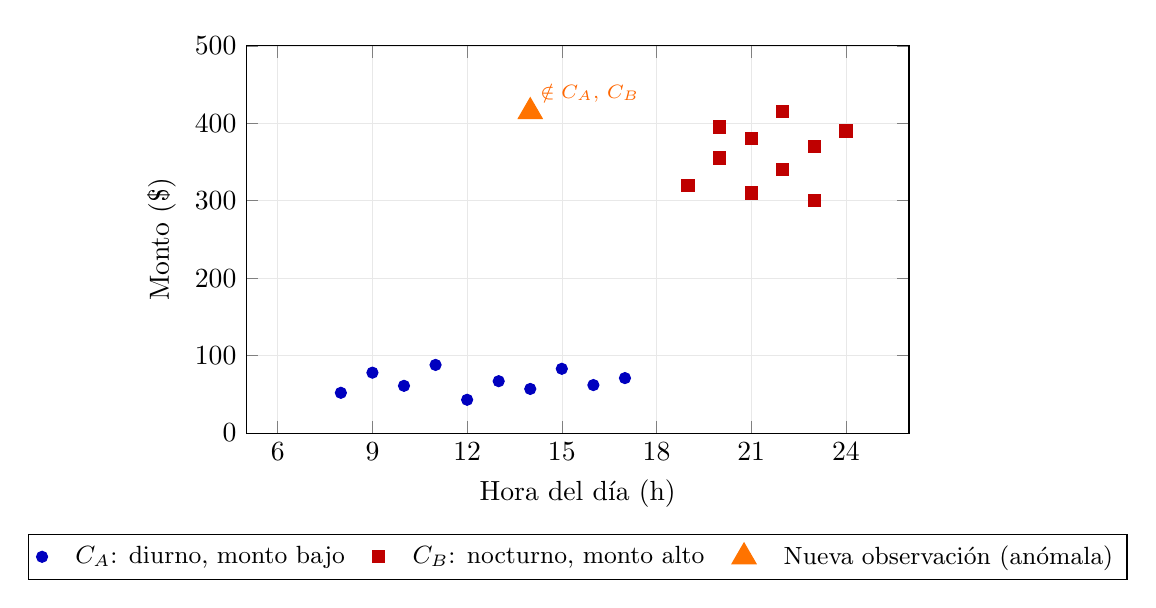
\begin{tikzpicture}
  \begin{axis}[
    xlabel={Hora del día (h)},
    ylabel={Monto (\$)},
    xmin=5, xmax=26,
    ymin=0, ymax=500,
    xtick={6,9,12,15,18,21,24},
    ytick={0,100,200,300,400,500},
    grid=major,
    grid style={gray!18, very thin},
    width=10cm, height=6.5cm,
    % Leyenda exterior: debajo del eje X
    legend style={
      at={(0.5,-0.26)},
      anchor=north,
      legend columns=3,
      font=\small,
      cells={anchor=west},
      column sep=8pt,
    },
  ]
  % --- Cluster A: diurno, monto bajo (horas 8-17) ---
  \addplot[only marks, mark=*, mark size=2pt, blue!75!black]
    coordinates {
      (8,52)(9,78)(10,61)(11,88)(12,43)
      (13,67)(14,57)(15,83)(16,62)(17,71)
    };
  \addlegendentry{$C_A$: diurno, monto bajo}

  % --- Cluster B: nocturno, monto alto (horas 19-24) ---
  \addplot[only marks, mark=square*, mark size=2.2pt, red!75!black]
    coordinates {
      (19,320)(20,355)(20,395)(21,310)(21,380)
      (22,340)(22,415)(23,370)(23,300)(24,390)
    };
  \addlegendentry{$C_B$: nocturno, monto alto}

  % --- Nueva observacion anomala: hora diurna, monto alto ---
  \addplot[only marks, mark=triangle*, mark size=5pt, orange!90!red]
    coordinates {(14,415)};
  \addlegendentry{Nueva observación (anómala)}

  % --- Etiqueta junto al punto anomalo ---
  \node[above right, font=\scriptsize, text=orange!80!red]
    at (axis cs:14,415) {$\notin C_A,\, C_B$};

  \end{axis}
\end{tikzpicture}
\caption{Flujo de transacciones bancarias procesadas por BIRCH. Los clusters $C_A$ (diurno, monto bajo) y $C_B$ (nocturno, monto alto) representan el conocimiento incremental acumulado. La nueva observación (14\,h, \$415) no supera el umbral de similitud $T$ con ninguno de los dos perfiles existentes, por lo que BIRCH crea un tercer nodo CF~\cite{zhang1996birch}.}
\label{fig:incremental}
\end{figure}

Cuando llega una transacción a las 14\,h con monto de \$415, su distancia al centroide de $C_A$ (monto $\approx\$66$, horas 8–17) supera el umbral $T$ por exceso de monto, y su distancia al centroide de $C_B$ (horas 19–24) lo supera por discrepancia horaria. BIRCH crea una nueva hoja en el árbol CF, dando origen a un tercer perfil potencialmente fraudulento, sin necesidad de reanálisis global~\cite{zhang1996birch}. La capacidad de adaptarse a patrones emergentes sin reentrenar desde cero es la propiedad que distingue a los algoritmos incrementales en entornos de datos en flujo~\cite{gama2014survey}.